\section{Weight decay Improves Language Model Plasticity}
\label{sec:exps}


We present the main experimental results. We begin by identifying the optimal pretraining weight decay based on pretraining performance (Section~\ref{subsec:exps-wd-ptloss}), a common way to select pretraining hyperparameters \citep{hoffmann2022training}. Next, we investigate how weight decay shapes the plasticity of the pretrained model and identify its optimal pretraining value based on downstream performance (Section~\ref{subsec:exps-wd-plasticity}). Then, we examine whether a model's pretraining performance is fully predictive of its downstream performance (Section~\ref{subsec:exps-ptloss-vs-ftperf}).



\subsection{The optimal pretraining weight decay based on pretraining validation loss} 
\label{subsec:exps-wd-ptloss}




\begin{figure*}[t]
    \centering
    \begin{subfigure}[b]{0.30\textwidth}
        \centering
        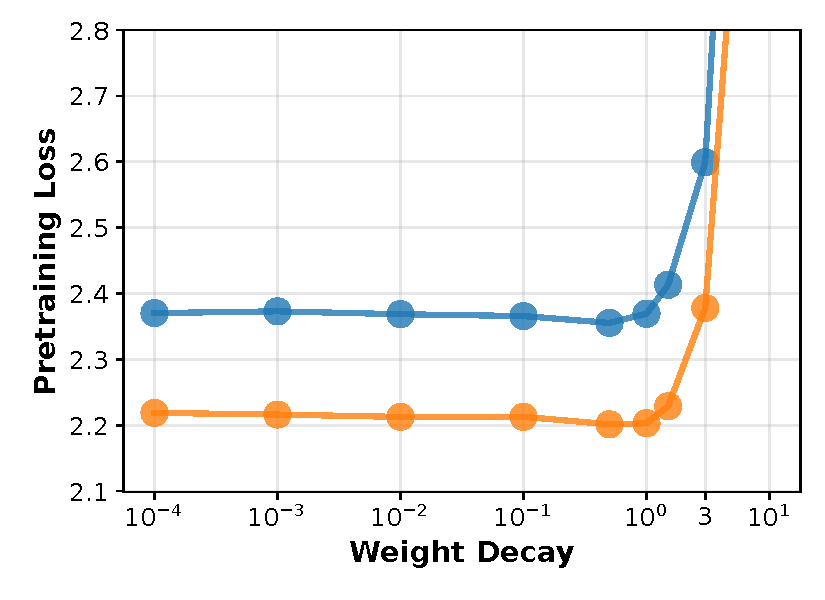
\includegraphics[width=\linewidth]{figs/a04_val_loss/new/wd_vs_loss_llamax2_nolegend.pdf}
        \caption{\llama{} at 20 TPP}
    \end{subfigure}
    \hfill
    \begin{subfigure}[b]{0.34\textwidth}
        \centering
        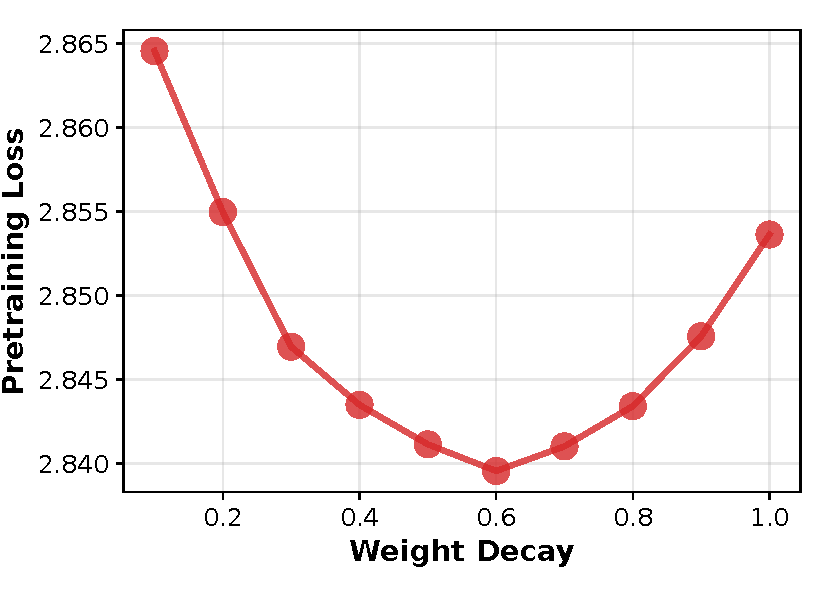
\includegraphics[width=0.88\linewidth]{figs/a04_val_loss/new/wd_vs_loss_zoomedin_OLMo-2-1B-20x_nolegend.pdf}
        \caption{\olmo{} at 20 TPP}
    \end{subfigure}
    \hfill
    \begin{subfigure}[b]{0.34\textwidth}
        \centering
        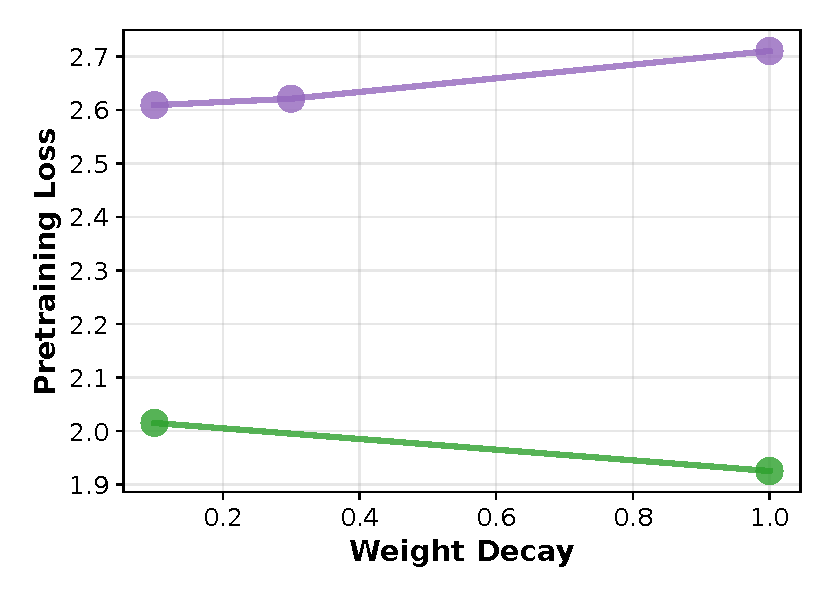
\includegraphics[width=0.88\linewidth]{figs/a04_val_loss/new/wd_vs_loss_zoomedin_Llama-2-4B-20x___OLMo-2-1B-140x_nolegend.pdf}
        \caption{\llama{} 4B and  \olmo{} at 140 TPP}
    \end{subfigure}$\,$\\[4pt]
            
\includegraphics[width=0.8\linewidth]{figs/a04_val_loss/new/wd_vs_loss_legend.pdf}
    \caption{{\bf Validation cross-entropy loss of models pretrained with different weight decay values.} The weight decay value that minimizes pretraining validation loss may be equal to or larger than the standard default value of 0.1 depending on the training regime.}
    \label{fig:wd-vs-pt-loss}
\end{figure*}



\begin{figure*}[h] 
    \centering
    \begin{subfigure}[b]{\textwidth} 
        \centering
        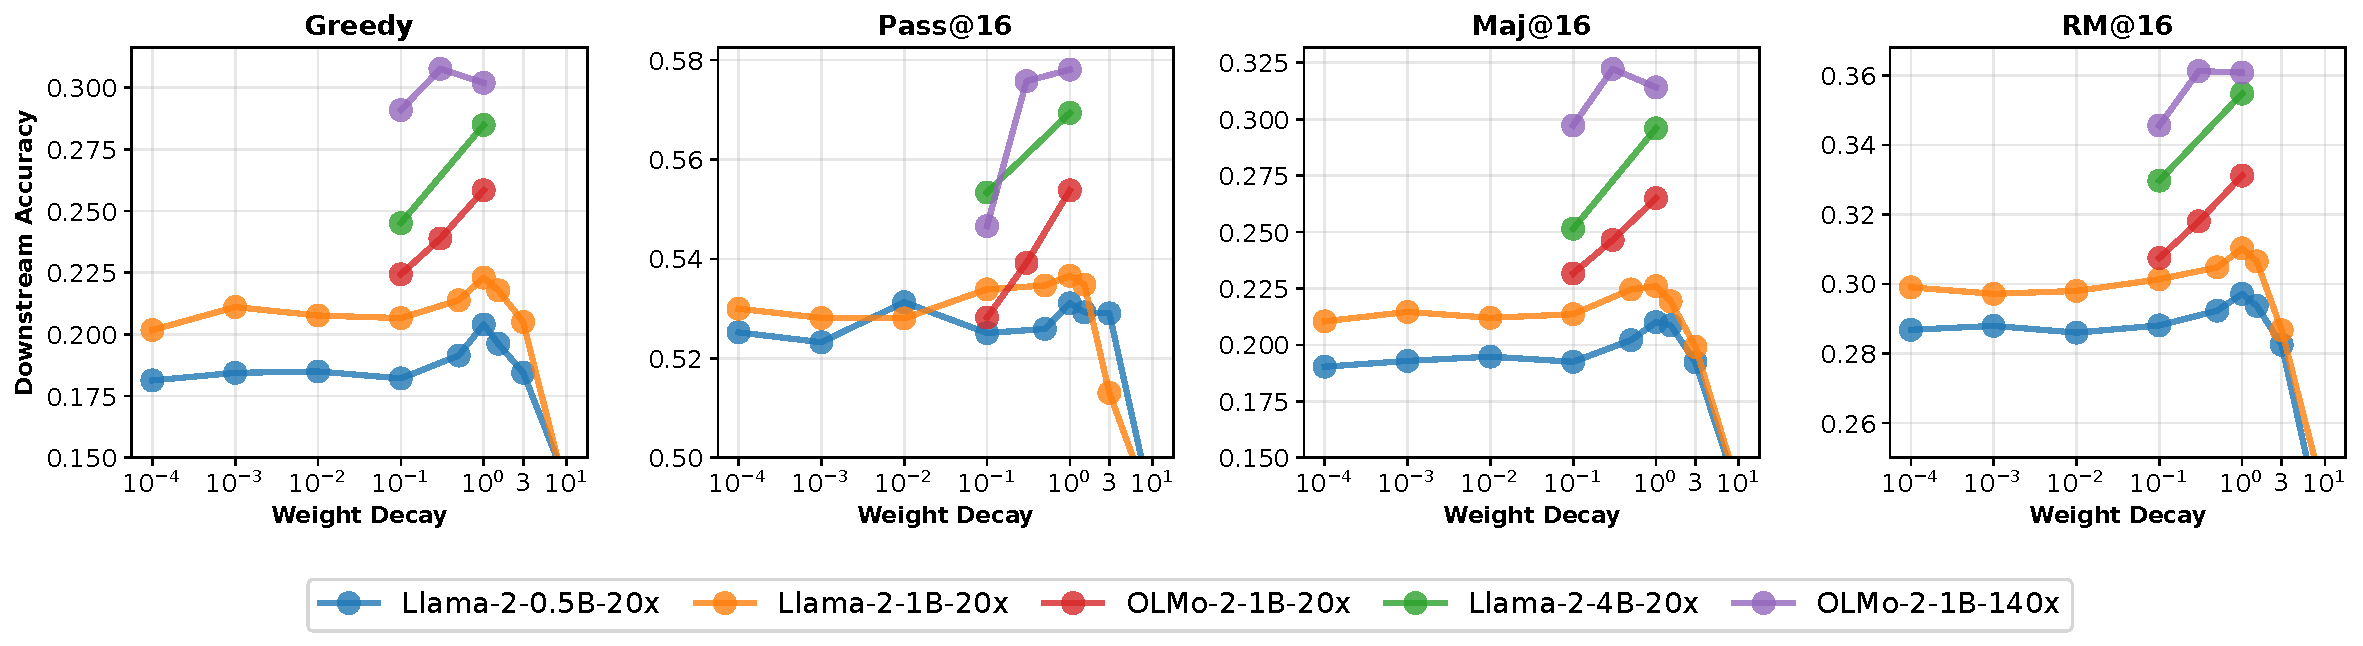
\includegraphics[width=\linewidth]{figs/a01_ft_cot/new/wd_vs_ft_perf_4metrics.pdf} 
    \end{subfigure}
    \caption{{\bf Weight decay during pretraining improves language model plasticity and downstream performance.} We pretrain models with different weight decay values and fine-tune them on various downstream tasks. This figure shows the average downstream performance for six chain-of-thought reasoning tasks. The results indicate that weight decay improves model plasticity and downstream performance. In these experiments, the optimal weight decay for downstream performance is larger than the standard default of 0.1. In addition, the optimal weight decay based on pretraining loss (Figure~\ref{fig:wd-vs-pt-loss}) and that based on downstream performance (this figure) are different, suggesting that optimizing hyperparameters based on pretraining loss alone does not always produce models with the best downstream performance.}
    \label{fig:wd-vs-ft-performance}
\end{figure*}


We first identify the weight decay value that leads to the lowest cross-entropy validation loss after pretraining. This is the value considered optimal by current approaches in hyperparameter optimization for language model pretraining \citep{bergsma2505powerlines}. We pretrain various models by sweeping over different weight decay values and fixing all other hyperparameters (the values for weight decay and other hyperparameters are listed in Appendix~\ref{app:pt}). The validation cross-entropy loss of these pretrained models is shown in Figure~\ref{fig:wd-vs-pt-loss}.




Small weight decay values ($<$ 0.1) during pretraining have little effect on pretraining loss (Figure~\ref{fig:wd-vs-pt-loss}a). In contrast, moderate-to-large values ([0.1, 3]) can either decrease or increase pretraining loss, depending on the setting (Figures~\ref{fig:wd-vs-pt-loss}a-c), while extremely large values (e.g., 10) can substantially degrade pretraining performance (Figure~\ref{fig:wd-vs-pt-loss}a). The observation that weight decay can lower pretraining performance is consistent with prior work on vision transformers~\citep{zhai2022scaling,abnar2021exploring}.
At 20 TPP, for both \llama{} and \olmo{} models, we find that the optimal weight decay parameter is larger than the default of 0.1. 
In particular, among the weight decay values examined, the optimal weight decay is 0.5 for \llamazeropointfiveB{} and \llamaoneB{} (Figure~\ref{fig:wd-vs-pt-loss}a), 0.6 for \olmoonex{} (Figure~\ref{fig:wd-vs-pt-loss}b), and 1.0 for \llamafourB{} (Figure~\ref{fig:wd-vs-pt-loss}c).
However, this relationship changes as training time increases. At 140 TPP, for the \olmosevenx{} model, the default value of 0.1 outperforms (leads to a lower validation loss than) larger values of 0.3 and 1.0 (Figure~\ref{fig:wd-vs-pt-loss}c). This result that overtrained models have a lower optimal weight decay is consistent with previous analyses on weight decay scaling laws which recommend decreasing the value of the weight decay hyperparameter as training time (TPP) increases to optimize for pretraining validation loss \citep{bergsma2505powerlines}.





\subsection{The optimal pretraining weight decay based on downstream performance}
\label{subsec:exps-wd-plasticity}



\begin{figure*}[t] 
    \centering
    \begin{subfigure}{\textwidth} 
        \centering
        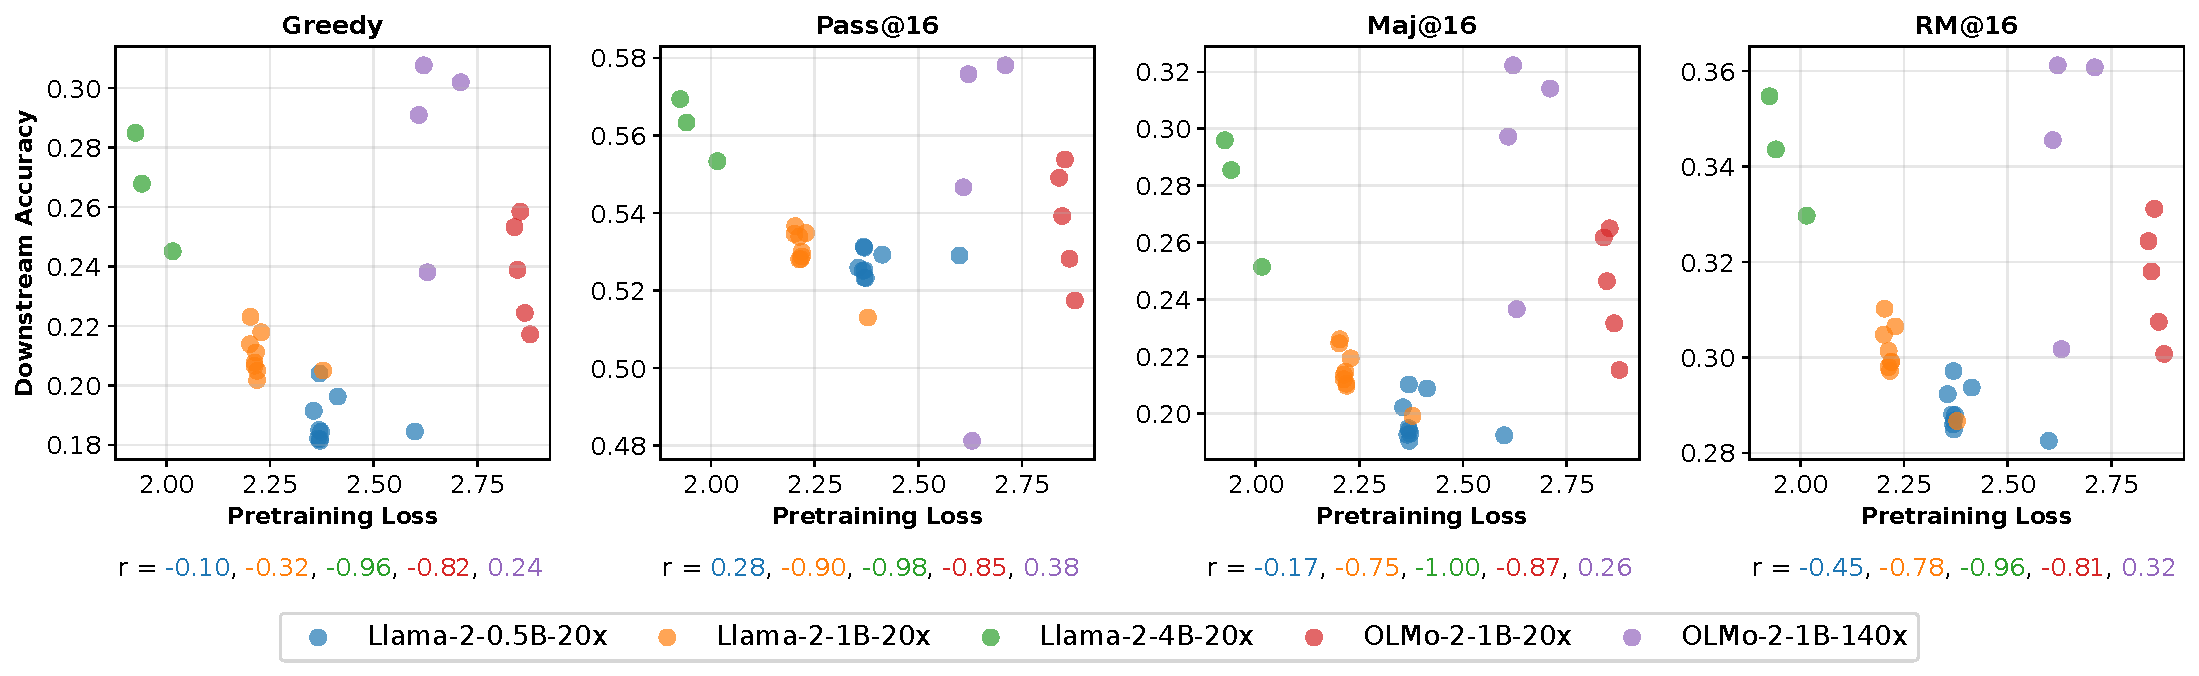
\includegraphics[width=\linewidth]{figs/a04_val_loss/new/all_models_loss_vs_ft_acc_all_datasets_4metrics.pdf}
    \end{subfigure}
    \caption{{\bf Pretraining performance is not perfectly predictive of downstream performance.} We examine the relationship between the models' pretraining validation cross-entropy loss (x-axis) and downstream accuracy on CoT reasoning tasks (y-axis). Better pretraining performance does not necessarily imply better downstream performance: while the two tend to be correlated, models with similar pretraining losses can perform differently downstream, and models with lower pretraining losses can perform better or worse downstream than models with higher pretraining losses. Thus, optimizing for pretraining loss alone may not always yield the best final model.}
    \label{fig:pt-loss-vs-ft-perf}
\end{figure*}

Next, we investigate how weight decay during pretraining affects model plasticity and downstream model performance.
We fine-tune the pretrained models from Section~\ref{subsec:exps-wd-ptloss} (which were trained with different weight decay values) on diverse downstream tasks spannning CoT reasoning, language understanding and commonsense reasoning, and safety alignment. Then, we evaluate the final models' performance on these tasks. 
The average downstream performance of the models after fine-tuning on CoT reasoning tasks is shown in Figure~\ref{fig:wd-vs-ft-performance}.
The downstream performance for other tasks is in Appendix~\ref{app:ft}.

Among models that achieved reasonable pretraining validation losses in Section~\ref{subsec:exps-wd-ptloss} (i.e., models that are suitable candidates for subsequent training), higher weight decay during pretraining confers a higher degree of model plasticity, enabling the pretrained model to learn better during fine-tuning and perform better on the fine-tuning task.
The results show that models pretrained with weight decay higher than the default 0.1 value perform better on downstream tasks. This finding is consistent across model families (\llama{} and \olmo{}), model sizes (up to 4B parameters), training regimes (20 TPP and 140 TPP), fine-tuning tasks (twelve tasks spanning CoT reasoning, language understanding and commonsense reasoning, and safety alignment), and evaluation metrics.
Examining the CoT reasoning tasks more closely, we observe that, among the weight decay values examined, in the compute-optimal 20 TPP regime, the optimal pretraining weight decay is 1.0 (\llamazeropointfiveB{}, \llamaoneB{}, \llamafourB{}, and \olmoonex{}). In the overtrained 140 TPP regime, the optimal pretraining weight decay is 0.3 (\olmosevenx{}). It is possible that, as models are trained for even longer (i.e., beyond 140 TPP), the optimal pretraining weight decay that leads to the best downstream model performance may continue to decrease (this would need to be confirmed with experiments at larger training scales). 




We also compare two notions of optimal weight decay: the weight decay value that minimizes pretraining validation cross-entropy loss (Figure~\ref{fig:wd-vs-pt-loss}), as is commonly used in current approaches~\citep{bergsma2505powerlines}, and the value that maximizes model performance after fine-tuning (Figure~\ref{fig:wd-vs-ft-performance}). We find that these two weight decay values differ for each model. We observe that the weight decay value that optimizes model performance after fine-tuning is higher (\llamazeropointfiveB{}, \llamaoneB{}, \olmoonex{}, \olmosevenx{}) or equivalent (\llamafourB{}) to the value that optimizes pretraining validation loss. This shows that the ``optimal'' weight decay during pretraining is not absolute -- it depends on the intended objective, such as optimizing for pretraining performance or downstream performance.



Does weight decay's effect on model plasticity depend on the choices of other hyperparameters? To investigate this, we perform experiments sweeping over pretraining and fine-tuning hyperparameters. We jointly vary weight decay and learning rate during pretraining and weight decay, learning rate, and batch size during fine-tuning. 
Details and results for these experiments are in Appendix~\ref{app:hyperparam-exps}.
Despite varying other hyperparameters, we find that models pretrained with higher weight decay consistently exhibit better downstream performance.
Thus, higher weight decay during pretraining consistently improves model plasticity and downstream performance across a range of pretraining and fine-tuning hyperparameter settings.

\begin{finding}
\textbf{Finding 1.} Pretraining weight decay can improve model plasticity and lead to better downstream performance. The optimal pretraining weight decay value for plasticity is larger than the default of 0.1.
\end{finding}







\subsection{The relationship between pretraining loss and downstream performance} 
\label{subsec:exps-ptloss-vs-ftperf}





Following the findings from the previous sections, we now investigate whether a model's pretraining performance is predictive of its downstream performance. 
We examine the pretraining validation cross-entropy loss of the pretrained models (from Section~\ref{subsec:exps-wd-ptloss}) and their downstream accuracy on CoT reasoning tasks after fine-tuning (from Section~\ref{subsec:exps-wd-plasticity}). The relationship between these two variables is plotted in Figure~\ref{fig:pt-loss-vs-ft-perf}. 

We compare models with the same training setup (i.e., same model family, size, and TPP) that differ only in the pretraining weight decay hyperparameter. Although better pretraining performance tends to be associated with better downstream performance\footnote{The correlations in Figure~\ref{fig:pt-loss-vs-ft-perf} should be interpreted as suggestive rather than conclusive, given the relatively small sample size of each model group ($n \leq 10$). However, the main takeaway (i.e., better pretraining loss does not necessarily lead to better downstream performance) does not depend on these correlations: in most model groups, there are cases where models with worse pretraining loss achieve better downstream performance, and models with similar pretraining loss perform differently downstream.}, pretraining performance is not a perfect proxy of downstream performance.
Sometimes, models with similar pretraining performance can perform differently downstream (such observations exist for \llamazeropointfiveB{}, \llamaoneB{}, and \olmoonex{}). 
In addition, models with better pretraining performance (lower pretraining validation loss) can perform better downstream (such observations exist for all five model groups) or worse downstream (such observations exist for \llamazeropointfiveB{}, \llamaoneB{}, and \olmosevenx{}).  
For example, \olmosevenx{} pretrained with weight decay 0.3 or 1.0 performs slightly worse after pretraining (achieving pretraining validation cross-entropy losses of 2.6208 and 2.7064, respectively) than the same model pretrained with weight decay 0.1 (which achieves a pretraining validation cross-entropy loss of 2.6088), but the former two pretrained models perform noticeably better after fine-tuning (Figure~\ref{fig:wd-vs-ft-performance}, purple line).
Altogether, these results show that pretraining performance is not perfectly predictive of downstream performance. As a result, optimizing for solely for pretraining loss may not always produce the best downstream (final) models.





\begin{finding}
\textbf{Finding 2.} The pretraining weight decay value that minimizes the pretraining cross-entropy validation loss does not necessarily lead to the best downstream performance.
\end{finding}



